\problemname{\problemyamlname}

\begin{wrapfigure}{r}{5.5cm}
    \centering
    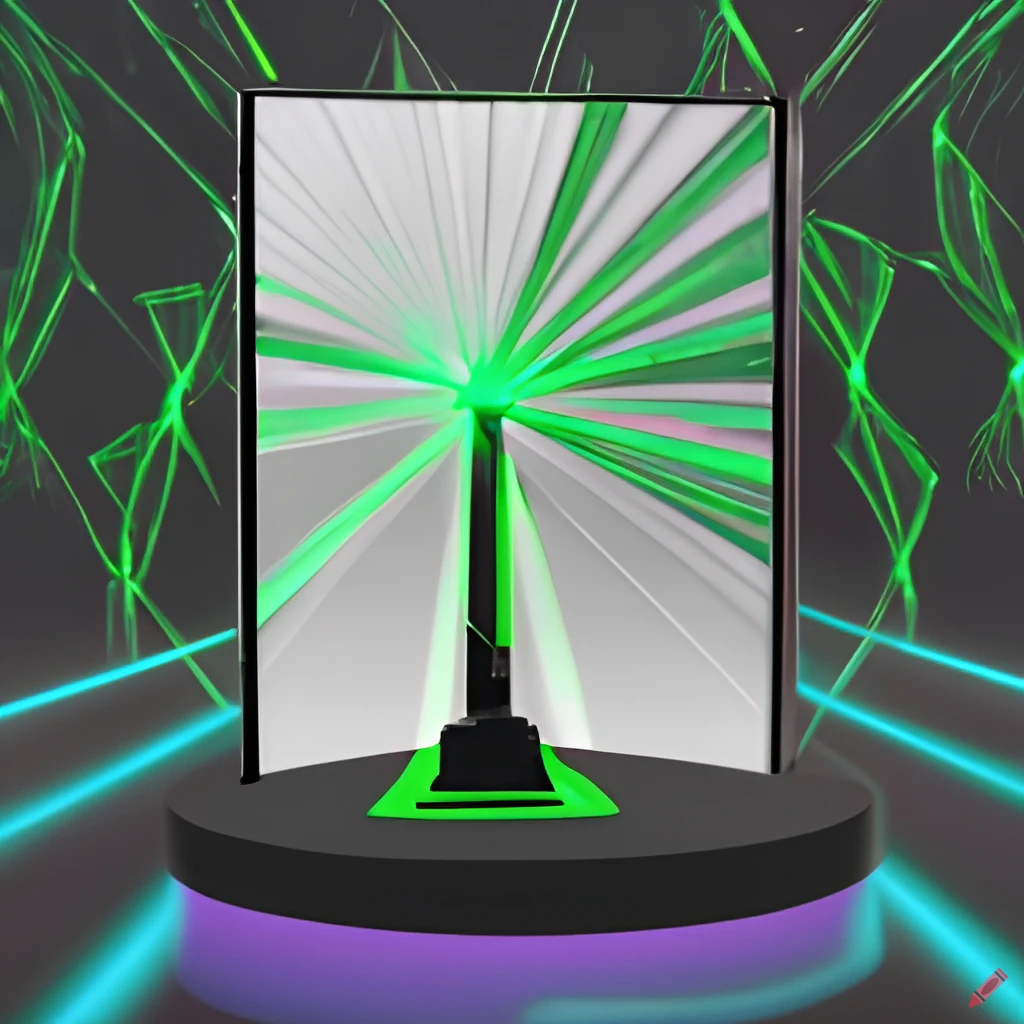
\includegraphics[width=5.5cm]{mirror.jpg}
\end{wrapfigure}
Ça y est, vous vous préparez pour aller au KARWa-au-quai annuel entre l'UCLouvain et l'UMons, événement incontournable de la vie étudiante, là où les vocations de chanteurs se créent, où tous les labels de musiques viennent repérer les futurs prodiges de demain.

Vous devez être au top de votre forme, tant dans votre chant que pour votre apparence.
Rien ne doit être laissé au hasard et vous comptez bien impressionner la totalité des personnes sobres de la salle\footnote{C'est-à-dire tout le monde, bien évidemment, cet événement est trop important pour boire avant la fin des chansons...} lorsque vous serez sur scène avec vos coéquipiers pour chanter en coeur.
En plus de chanter, vous avez préparé un petit jeu de laser et de lumière via des miroirs pour éblouir la salle.

Sur scène, un de vos coéquipiers et vous serez sur une même ligne, face au public.
Derrière vous, un grand miroir sera parallèle à cette ligne.
Vous connaissez la distance directe (perpendiculaire) entre votre position et le miroir,
et vous allez activer un faisceau laser depuis votre position vers le miroir avec un angle
précis par rapport à la perpendiculaire, de sorte que le laser rebondisse sur votre coéquipier.
Vous devez déterminer la distance à laquelle votre coéquipier devra se tenir afin qu'il réceptionne parfaitement le faisceau laser.

\begin{Input}
	L'entrée consiste en :
	\begin{itemize}
		\item une ligne contenant un entier $d$ ($0 < d \le 10^6$), la distance qui vous sépare du miroir,
		\item une ligne contenant un entier $\alpha$ ($0 < \alpha < 90$), l'angle en degré avec lequel vous allez projeter le laser sur le miroir (si $\alpha=0$, vous vous visez vous-même dans le miroir, si $\alpha=90$, vous visez votre coéquipier sans toucher le miroir).
	\end{itemize}
\end{Input}

\begin{Output}
	La distance entre votre coéquipier et vous afin qu'il reçoive le laser sur lui.
	La réponse doit avoir une erreur absolue ou relative de maximum $10^{-6}$.
\end{Output}
